\documentclass[a4paper,12pt]{article}

\usepackage[T2A]{fontenc}			
\usepackage[utf8]{inputenc}			
\usepackage[english,russian]{babel}	

\usepackage[
bookmarks=true, colorlinks=true, unicode=true,
urlcolor=black,linkcolor=black, anchorcolor=black,
citecolor=black, menucolor=black, filecolor=black,
]{hyperref}

\usepackage{color}
\usepackage{caption}
\DeclareCaptionFont{white}{\color{black}}
\DeclareCaptionFormat{listing}{\colorbox{white}{\parbox{\textwidth}{#1#2#3}}}
\captionsetup[lstlisting]{format=listing,labelfont=white,textfont=white}

\usepackage{amsmath,amsfonts,amssymb,amsthm,mathtools} 
\usepackage{wasysym}

\usepackage{graphicx}
%\usepackage[cache=false]{minted}
\usepackage{cmap}
\usepackage{indentfirst}

\usepackage{listings} 
\usepackage{fancyvrb}

\usepackage{geometry}
\geometry{left=2cm}
\geometry{right=1.5cm}
\geometry{top=1cm}
\geometry{bottom=2cm}

\setlength{\parindent}{5ex}
\setlength{\parskip}{0.5em}

\usepackage{pgfplots}
\usetikzlibrary{datavisualization}
\usetikzlibrary{datavisualization.formats.functions}

\begin{document}
	\lstset{ %
		language=C,                 % выбор языка для подсветки (здесь это С)
		basicstyle=\small\sffamily, % размер и начертание шрифта для подсветки кода
		numbers=left,               % где поставить нумерацию строк (слева\справа)
		numberstyle=\tiny,           % размер шрифта для номеров строк
		stepnumber=1,                   % размер шага между двумя номерами строк
		numbersep=5pt,                % как далеко отстоят номера строк от подсвечиваемого кода
		backgroundcolor=\color{white}, % цвет фона подсветки - используем \usepackage{color}
		showspaces=false,            % показывать или нет пробелы специальными отступами
		showstringspaces=false,      % показывать или нет пробелы в строках
		showtabs=false,             % показывать или нет табуляцию в строках
		frame=single,              % рисовать рамку вокруг кода
		tabsize=2,                 % размер табуляции по умолчанию равен 2 пробелам
		captionpos=t,              % позиция заголовка вверху [t] или внизу [b] 
		breaklines=true,           % автоматически переносить строки (да\нет)
		breakatwhitespace=false, % переносить строки только если есть пробел
		escapeinside={\%*}{*)}   % если нужно добавить комментарии в коде
	}
	
	% Титульный лист
	\begin{figure}[h!]
		\begin{center}
			{
\includegraphics[scale = 0.4]{titul.jpg}}
			\label{titul}
		\end{center}
	\end{figure}
	
	\vspace*{15mm} 
	
	\huge
	\begin{center}
		Дисциплина: <<Функциональное и логическое программирование>>
	\end{center}
	\vspace*{15mm} 	
	
	\begin{center}
		Лабораторная работа №9
	\end{center}
	
	\vspace*{15mm} 	
	
	\large
	\begin{flushright}
		Студент: Левушкин И. К. \\
		Группа: ИУ7-62Б \\
		Преподаватели: Толпинская Н. Б., \\ Строганов Ю. В. \\
	\end{flushright}
	
	\vspace*{30mm}
	\begin{center}
		Москва, 2020 г.  
	\end{center}
	\thispagestyle{empty}
	
	
	\newpage
	
	\section*{5.2. Написать предикат set-equal, который возвращает t, если два его множество-аргумента содержат одни и те же элементы, порядок которых не имеет значения.
	 }
 
 	\textit{Примечание: под множеством я понимаю список НЕПОВТОРЯЮЩИХСЯ элементов, порядок которых не имеет значения}
 	
 	Поскольку в скинутой Натальей Борисовной лекции есть пример преобразования списка в множество, где элементы в результате не повторяются:
 	
 	\begin{figure}[h!]
 		\begin{center}
 			{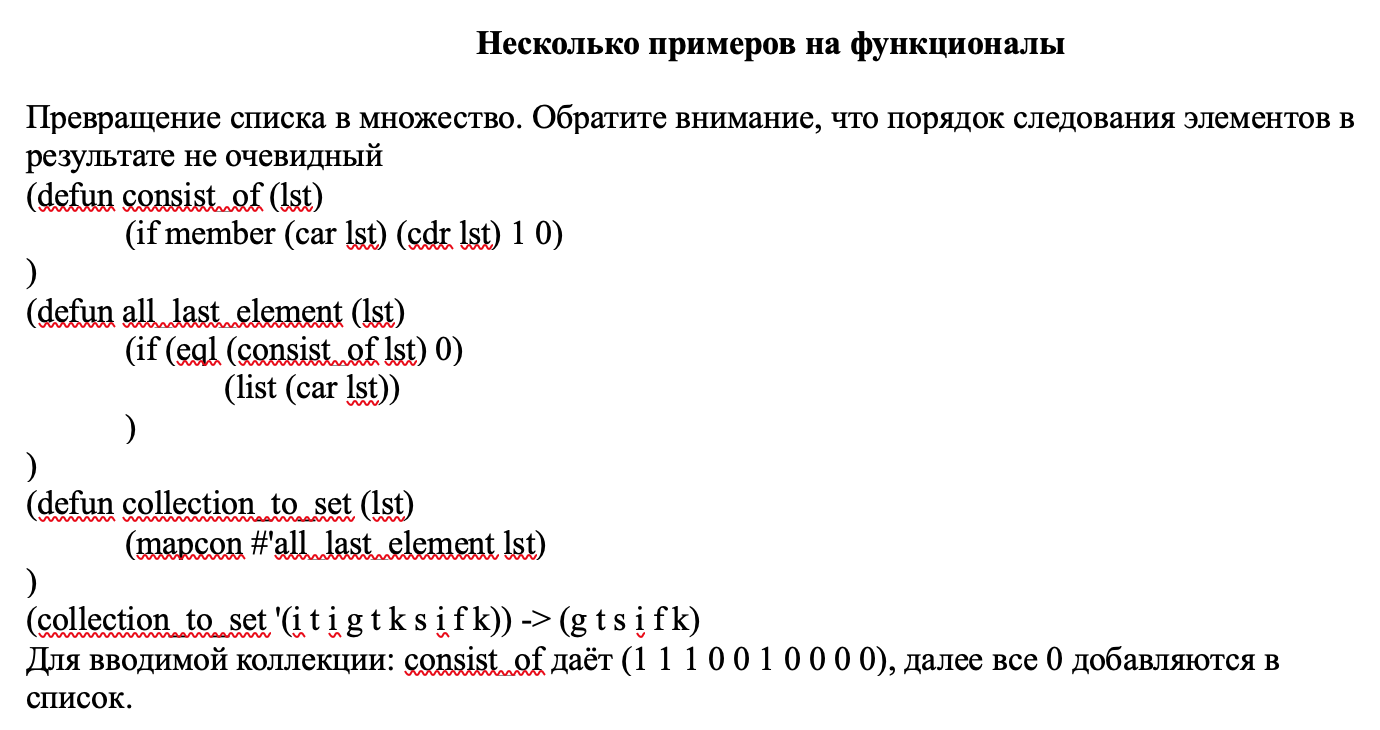
\includegraphics[scale = 0.7]{set.png}}
 			\label{ris:set}
 		\end{center}
 		\caption{Пример множества из лекции по рекурсии}
 	\end{figure}
 	
 	\newpage
 
 	\subsection*{Реализация задания}
 	
 	\begin{figure}[h!]
 		\begin{center}
 			{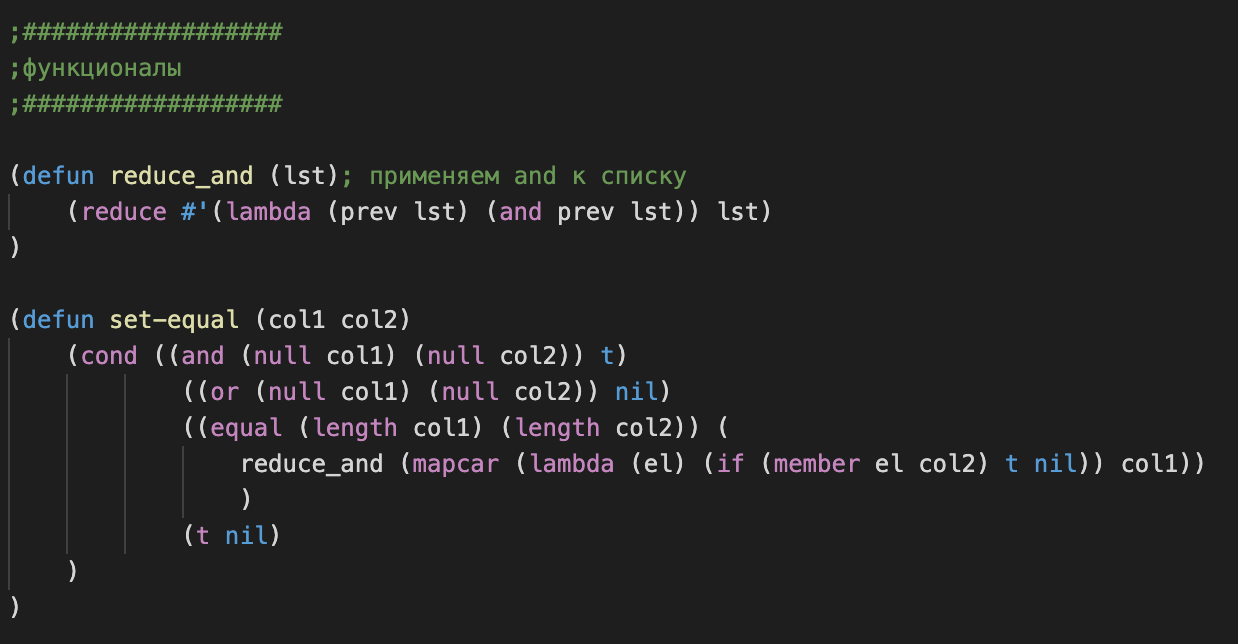
\includegraphics[scale = 0.8]{5.2f.png}}
 			\label{ris:5.2f}
 		\end{center}
 	\caption{Реализация функции set-equal с использованием функционалов}
 	\end{figure}
 
  	\begin{figure}[h!]
 	\begin{center}
 		{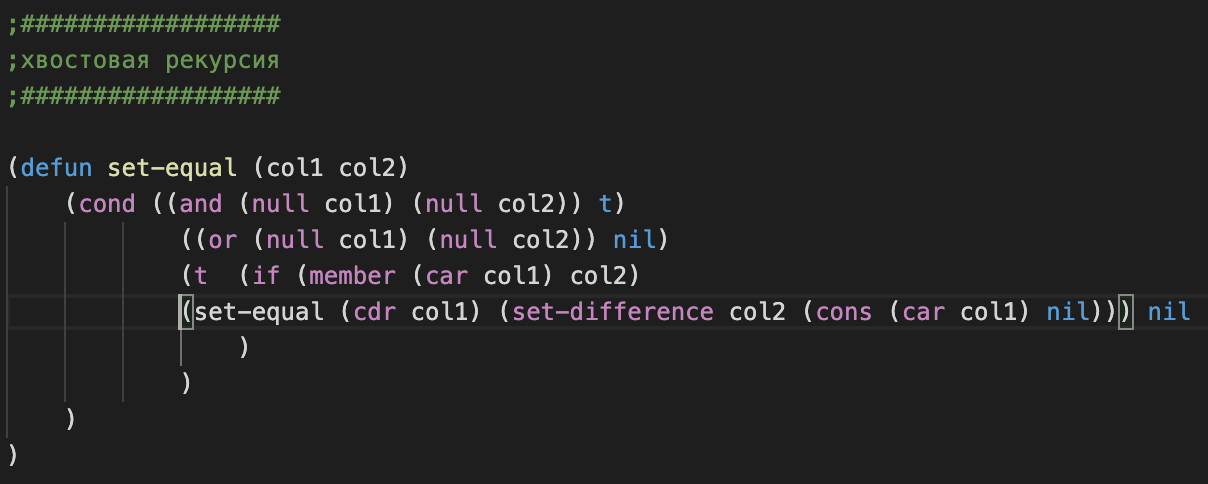
\includegraphics[scale = 0.8]{5.2r.png}}
 		\label{ris:5.2r}
 	\end{center}
 \caption{Рекурсивная реализация фунции set-equal}
 \end{figure}
 	
 	\newpage
 	
 	\subsection*{Назначение параметров функций}
 	
 	\begin{itemize}
 		\item Функция reduce\_and применяет and к списку
 		\item Функция member проверяет, есть ли элемент el в списке col2
 		\item Функция set\_difference получает на выходе разницу между списком col2 и головой списка col1
 	\end{itemize}
 	
 	\subsection*{Результаты работы}
 	
 	Функции, реализованные с помощью функционалов и с помощью хвостовой рекурсии выдают одинаковые результаты на одних и тех же параметрах:
 	
 	\begin{table} [h!]
 		\begin{center}
 			\begin{tabular}{|l|l|}
 				\hline
 				{\bf  Выражение} & {\bf Результат} \\
 				\hline
 				{'(1 2 3 4 5) '(4 3 2 5 1)} & T\\
 				\hline
 				{'(1 2 3 4 5 5 4 3 2 1) '(4 3 2 5 1)} & NIL\\
 				\hline
 				{'(1 2 3) '(1 2)} & NIL\\
 				\hline
 				{'(1) '(1)} & T\\
 				\hline
 				{'() '()} & T\\
 				\hline
 			\end{tabular}  
 			\label{m1}
 		\end{center}
 	\end{table}
 	
 	\newpage
 	
 	\section*{5.3. Напишите необходимые функции, которые обрабатывают таблицу из точечных пар:
(страна. столица), и возвращают по стране - столицу, а по столице - страну.
 	}
 	
 	\subsection*{Реализация задания}
 	
 	\begin{figure}[h!]
 		\begin{center}
 			{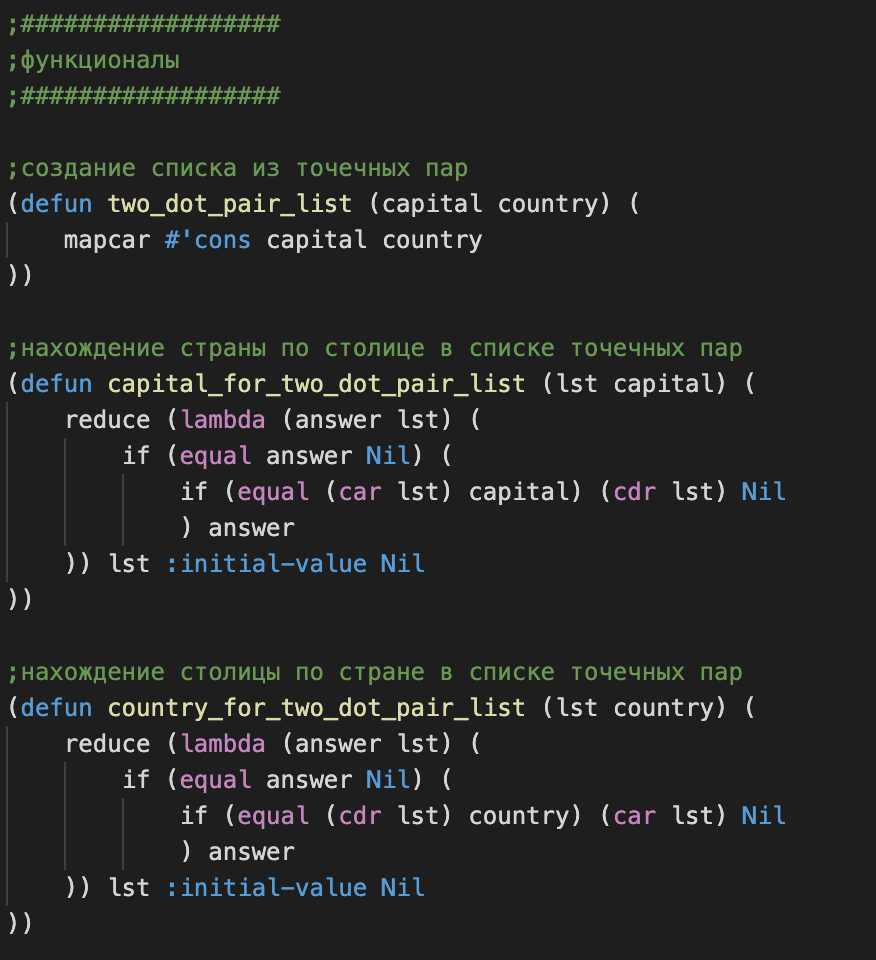
\includegraphics[scale = 1.0]{5.3f.png}}
 			\label{ris:5.3f}
 		\end{center}
 	\caption{Реализация функций с использованием функционалов}
 	\end{figure}
 
 	\newpage
 
  	\begin{figure}[h!]
 	\begin{center}
 		{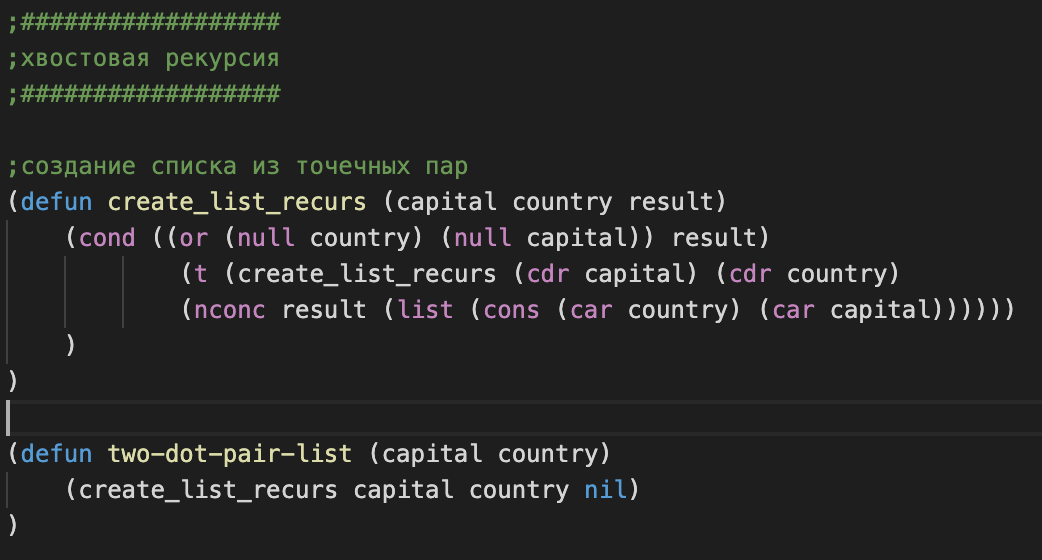
\includegraphics[scale = 0.8]{5.3r1.png}}
 		\label{ris:5.3r1}
 	\end{center}
 \caption{Рекурсивная реализация функций создания списка точечных пар}
 \end{figure}


 	\begin{figure}[h!]
	\begin{center}
		{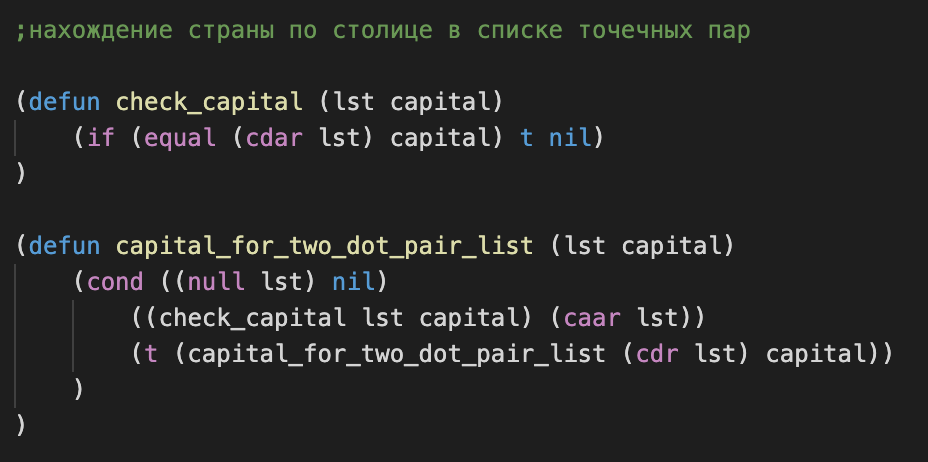
\includegraphics[scale = 0.9]{5.3r2.png}}
		\label{ris:5.3r2}
	\end{center}
\caption{Рекурсивная реализация функций нахождения страны по столице в списке точечных пар}
	\end{figure}


 	\begin{figure}[h!]
	\begin{center}
		{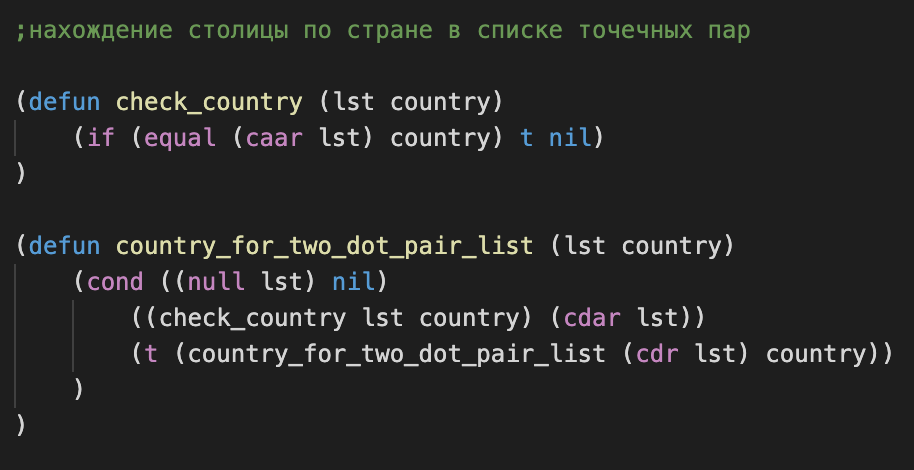
\includegraphics[scale = 0.9]{5.3r3.png}}
		\label{ris:5.3r3}
	\end{center}
\caption{Рекурсивная реализация функций нахождения столицы по стране в списке точечных пар}
\end{figure}
	
	\newpage
 	
 	\subsection*{Назначение параметров функций}
 	
 	 \begin{itemize}
 		\item Функция two\_dot\_pair\_list создает список точечных пар
 		\item Функция capital\_for\_two\_dot\_pair\_list ищет страну (второй элемент точечной пары) по столице (первый элемент точечной пары)
 		\item Функция country\_for\_two\_dot\_pair\_list ищет столицу (первый элемент точечной пары) по стране (второй элемент точечной пары)
 	\end{itemize}
 	
 	\textit{Описание функционалов:}
 	В предыдущих двух функциях используется функция reduce с начальным значением Nil, чтобы иметь возможность накапливать полученный результат в лямбда-функции в первом параметре.
 
 	\textit{Описание хвостовой рекурсии}
 	\begin{itemize}
 		\item Функция create\_list\_recurs является рекурсивной реализацией поставленной задачи, накапливая результат в result (two-dot-pair-list - оберточная функция)
 		\item Функция check\_capital сравнивает столицу capital со столицей в точечной паре головы списка lst
 	\end{itemize}
 	
 	\subsection*{Результаты работы}
 	
 	 	Функции, реализованные с помощью функционалов и с помощью хвостовой рекурсии выдают одинаковые результаты на одних и тех же параметрах:
 	
 	
 	\begin{table} [h!]
 		\begin{center}
 			\begin{tabular}{|l|l|}
 				\hline
 				{\bf  Выражение} & {\bf Результат two\_dot\_pair\_list}\\
 				\hline
 				{'(1 2 3 4 5 6) '(a b c d e f)} & ((1 . A) (2 . B) (3 . C) (4 . D) (5 . E) (6 . F))\\
 				\hline
 				{'(1 2 3 4 5 6) '(a b c d e)} & ((1 . A) (2 . B) (3 . C) (4 . D) (5 . E))\\
 				\hline
 				{'(1 2 3 4 5 6) '(a b c d e f g)} & ((1 . A) (2 . B) (3 . C) (4 . D) (5 . E) (6 . F))\\
 				\hline
 				{'() '()} & NIL\\
 				\hline
 			\end{tabular}  
 			\label{m2}
 		\end{center}
 	\end{table}
 
 \begin{table} [h!]
 	\begin{center}
 		\begin{tabular}{|l|l|}
 			\hline
 			{\bf  Выражение} & {\bf Результат capital\_for\_two\_dot\_pair\_list}\\
 			\hline
 			{'((1 . A) (2 . B) (3 . C) (4 . D) (5 . E) (6 . F)) 1} & A\\
 			\hline
 			{'((1 . A) (2 . B) (3 . C) (4 . D) (5 . E) (6 . F)) 5} & E\\
 			\hline
 			{'((1 . A) (2 . B) (3 . C) (4 . D) (5 . E) (6 . F)) 7} & NIL\\
 			\hline
 			{'((1 . A) (2 . B) (3 . C) (4 . D) (5 . E) (6 . F)) 'A} & NIL\\
 			\hline
 		\end{tabular}  
 		\label{m2}
 	\end{center}
 \end{table}

\begin{table} [h!]
	\begin{center}
		\begin{tabular}{|l|l|}
			\hline
			{\bf  Выражение} & {\bf Результат country\_for\_two\_dot\_pair\_list}\\
			\hline
			{'((1 . A) (2 . B) (3 . C) (4 . D) (5 . E) (6 . F)) 'A} & 1\\
			\hline
			{'((1 . A) (2 . B) (3 . C) (4 . D) (5 . E) (6 . F)) 'E} & 5\\
			\hline
			{'((1 . A) (2 . B) (3 . C) (4 . D) (5 . E) (6 . F)) 'G} & NIL\\
			\hline
			{'((1 . A) (2 . B) (3 . C) (4 . D) (5 . E) (6 . F)) 1} & NIL\\
			\hline
		\end{tabular}  
		\label{m2}
	\end{center}
\end{table}
 	
 	\newpage
 	
 	\section*{5.7. Напишите функцию, которая умножает на заданное число-аргумент все числа
из заданного списка-аргумента, когда
 	}
 	
 	\begin{enumerate}
 		\item все элементы списка --- числа,
 		\item элементы списка -- любые объекты.
 	\end{enumerate}
 	
 	
 	\subsection*{Реализация задания}
 	
 	\begin{figure}[h!]
 		\begin{center}
 			{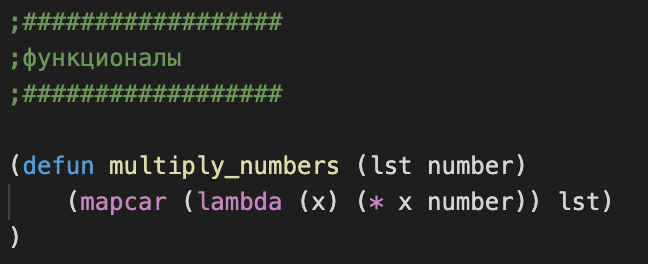
\includegraphics[scale = 1.3]{5.7f.png}}
 			\label{ris:5.7f}
 		\end{center}
 	\caption{Реализация функции multiply\_numbers с использованием функционалов}
 	\end{figure}
 
  	\begin{figure}[h!]
 	\begin{center}
 		{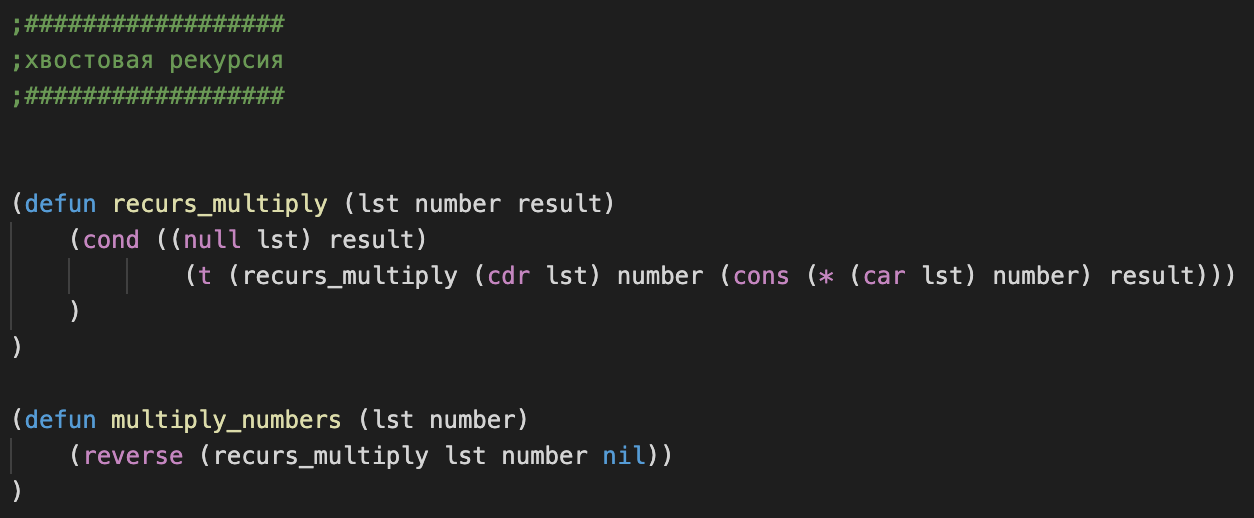
\includegraphics[scale = 0.8]{5.7r.png}}
 		\label{ris:5.7r}
 	\end{center}
 \caption{Рекурсивная реализация функции multiply\_numbers}
 \end{figure}

 	\newpage

 	\begin{figure}[h!]
	\begin{center}
		{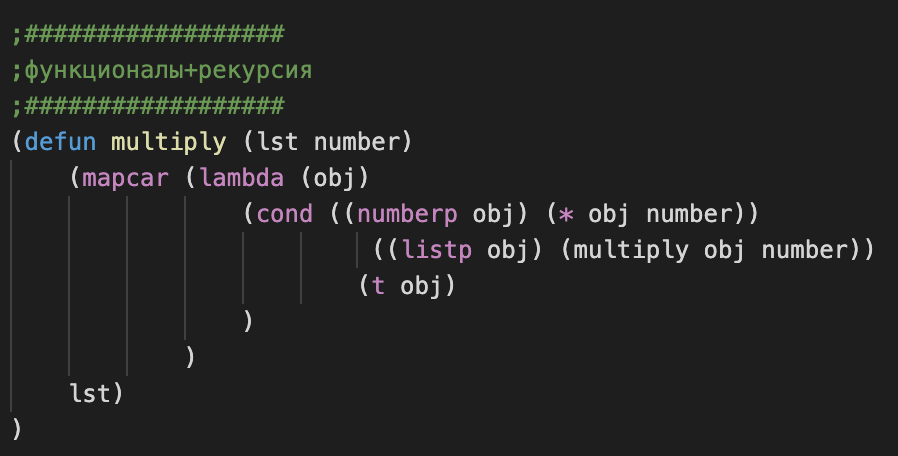
\includegraphics[scale = 1.0]{5.7rf.png}}
		\label{ris:5.7rf}
	\end{center}
\caption{Реализация функции multiply с использованием функционалов и рекурсии}
\end{figure}

 	
 	\subsection*{Назначение параметров функций}
 	
 	\begin{itemize}
 		\item Функции multiply\_numbers умножают на заданное число-аргумент все числа из заданного списка-аргумента, когда все элементы --- числа
 		\item Функция recurs\_multiply является рекурсивной реализацией поставленной задачи, накапливая результат в result (multiply\_numbers - оберточная функция)
 		\item Функция multiply умножаетт на заданное число-аргумент все числа из заданного списка-аргумента, когда все элементы --- любые объекты, причем использует она как функционалы, так и хвостовую рекурсию.
 	\end{itemize}
 	
 	\subsection*{Результаты работы}
 	
 	 	Функции, реализованные с помощью функционалов и с помощью хвостовой рекурсии выдают одинаковые результаты на одних и тех же параметрах:
 	
 	\begin{table} [h!]
 		\begin{center}
 			\begin{tabular}{|l|l|l|}
 				\hline
 				{\bf  Выражение} & {\bf Результат multiply\_numbers} & {\bf Результат multiply} \\
 				\hline
 				{'(1 2 3 4 5 6) 3} & (3 6 9 12 15 18) & (3 6 9 12 15 18)\\
 				\hline
 				{'(1 2 3 4 5 6) 0} & (0 0 0 0 0 0) & (0 0 0 0 0 0)\\
 				\hline
 				{'(1 2 3 4 5 6) 1} & (1 2 3 4 5 6) & (1 2 3 4 5 6)\\
 				\hline
 				{'() 5} & NIL & NIL\\
 				\hline
 				{'(1 2 3 (1 2) 4 5) 4} & --- & (4 8 12 (4 8) 16 20)\\
 				\hline 
 				{'(1 2 3 (1 2 (a 3)) 4 5) 6} & --- & (6 12 18 (6 12 (A 18)) 24 30)\\
 				\hline
 			\end{tabular}  
 			\label{m2}
 		\end{center}
 	\end{table}
 	
 	
 	\newpage
 	
 	\section*{6.2. Напишите функцию, которая уменьшает на 10 все числа из списка
аргумента этой функции.
 	}
 	
 	\subsection*{Реализация задания}
 	
 	Так как в условии задачи не сказано, является ли список-аргумент списком чисел, будем считать, что элементы списка - любые объекты:
 	
 	\begin{figure}[h!]
 		\begin{center}
 			{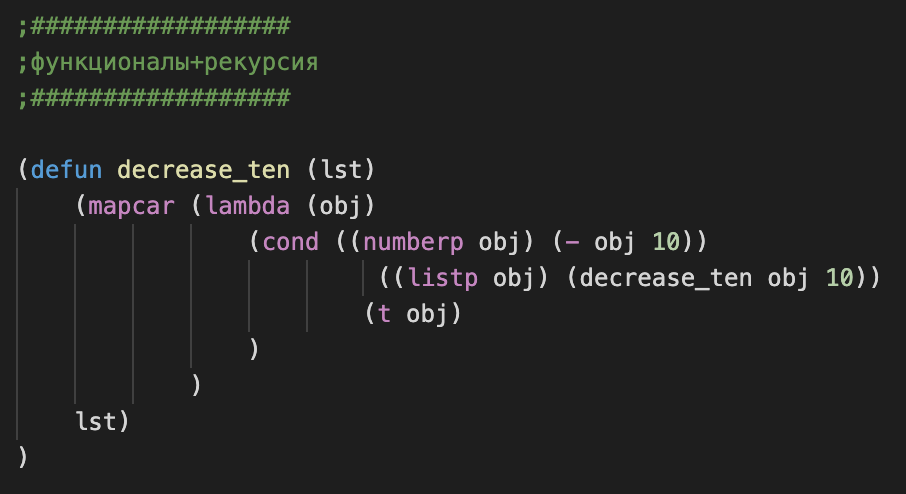
\includegraphics[scale = 1.0]{6.2.png}}
 			\label{ris:6.2}
 		\end{center}
 	\caption{Реализация функции decrease\_ten с использованием функционалов и рекурсии}
 	\end{figure}
 	
 	\subsection*{Назначение параметров функций}
 	
 	\begin{itemize}
 		\item Функция decrease\_ten по своей логике аналогична предыдущей функции multiply. Она также использует функционалы и хвстовую рекурсию.
 	\end{itemize}
 	
 	\subsection*{Результаты работы}
 	
 	\begin{table} [h!]
 		\begin{center}
 			\begin{tabular}{|l|l|}
 				\hline
 				{\bf  Выражение} & {\bf Результат} \\
 				{'(1 2 3 4 5 6)} & (-9 -8 -7 -6 -5 -4)\\
 				\hline
 				{'()} & NIL\\
 				\hline
 				{'(1 2 3 (1 2) 4 5)} & (-9 -8 -7 (-9 -8) -6 -5)\\
 				\hline 
 				{'(1 2 3 (1 2 (a 3)) 4 5)} & (-9 -8 -7 (-9 -8 (A -7)) -6 -5)\\
 			\end{tabular}  
 			\label{m2}
 		\end{center}
 	\end{table}
 	
 	
 	\newpage
 	
 	\section*{6.3. Написать функцию, которая возвращает первый аргумент списка-аргумента, который сам является непустым списком.
 	}
 	
 	\subsection*{Реализация задания}
 	
 	\begin{figure}[h!]
 		\begin{center}
 			{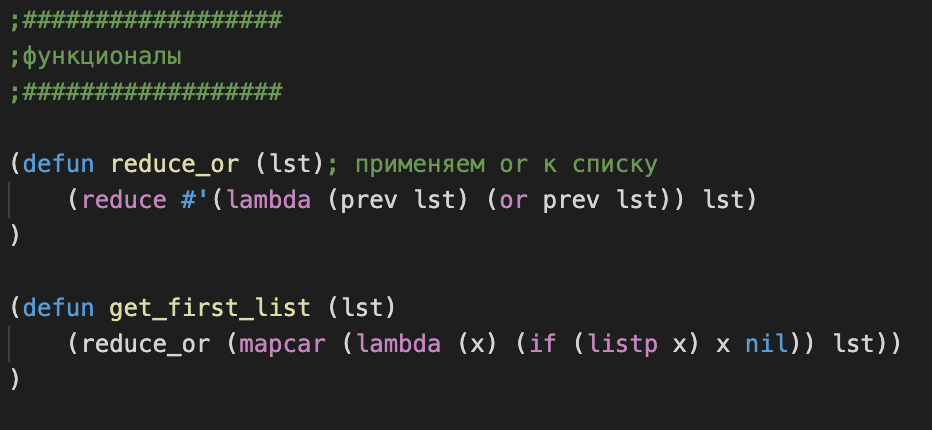
\includegraphics[scale = 1.0]{6.3f.png}}
 			\label{ris:6.3f}
 		\end{center}
 	\caption{Реализация функции, возвращающей первый непустой список-аргумент списка-аргумента, с использованием функционалов}
 	\end{figure}
 
 
  	\begin{figure}[h!]
 	\begin{center}
 		{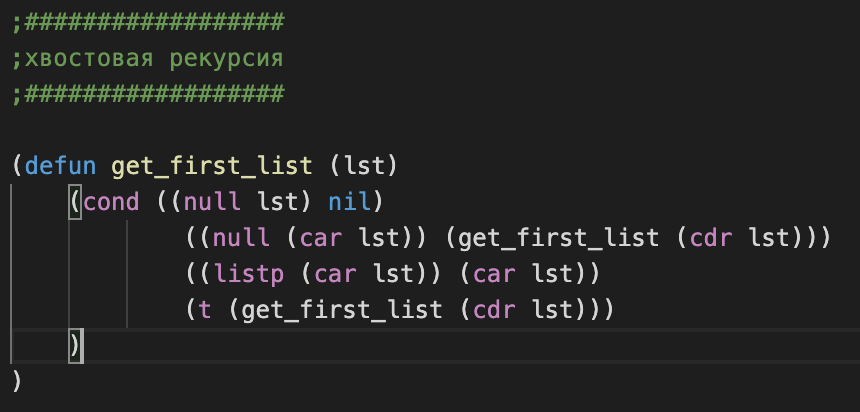
\includegraphics[scale = 1.0]{6.3r.png}}
 		\label{ris:6.3r}
 	\end{center}
 \caption{Рекурсивная реализация функции, возвращающей первый непустой список-аргумент списка-аргумента}
 \end{figure}
 	
 	\newpage
 	
 	\subsection*{Назначение параметров функций}
 	
 	\begin{itemize}
 		\item Функция reduce\_or применяет or на список lst
 		\item Функции get\_first\_list возвращает первый список-аргумент списка-аргумента
 		\item Для проверки элемента, является ли он списком или нет, используется функция listp
 		\item В рекурсивной реализации, чтобы возвращался не пустой список, присутствует дополнительная проверка на nil (второе условие в cond)
 	\end{itemize}
 	
 	\subsection*{Результаты работы}
 	
 	Функции, реализованные с помощью функционалов и с помощью хвостовой рекурсии выдают одинаковые результаты на одних и тех же параметрах:
 	
 	\begin{table} [h!]
 		\begin{center}
 			\begin{tabular}{|l|l|}
 				\hline
 				{\bf  Выражение} & {\bf Результат} \\
 				\hline
 				{'(1 2 3 4 5 6)} & NIL\\
 				\hline
 				{'(1 2 3 4 5 (1 2) (3 4) 6)} & (1 2)\\
 				\hline
 				{'(1 2 3 4 NIL (1 2) 5 6)} & (1 2)\\
 				\hline
 				{'()} & NIL\\
 				\hline
 			\end{tabular}  
 			\label{m2}
 		\end{center}
 	\end{table}
 	
 	
 	\newpage
 	
 	\section*{6.4. Написать функцию, которая выбирает из заданного списка только те числа,
которые больше 1 и меньше 10. (Вариант: между двумя заданными границами. )
 	}
 	
 	\subsection*{Реализация задания}
 	
 	Так как в условии задачи не сказано, является ли список-аргумент списком чисел, будем считать, что элементы списка - любые объекты.
 	Ниже представлен вариант для заданных двух границ:
 	
 	\begin{figure}[h!]
 		\begin{center}
 			{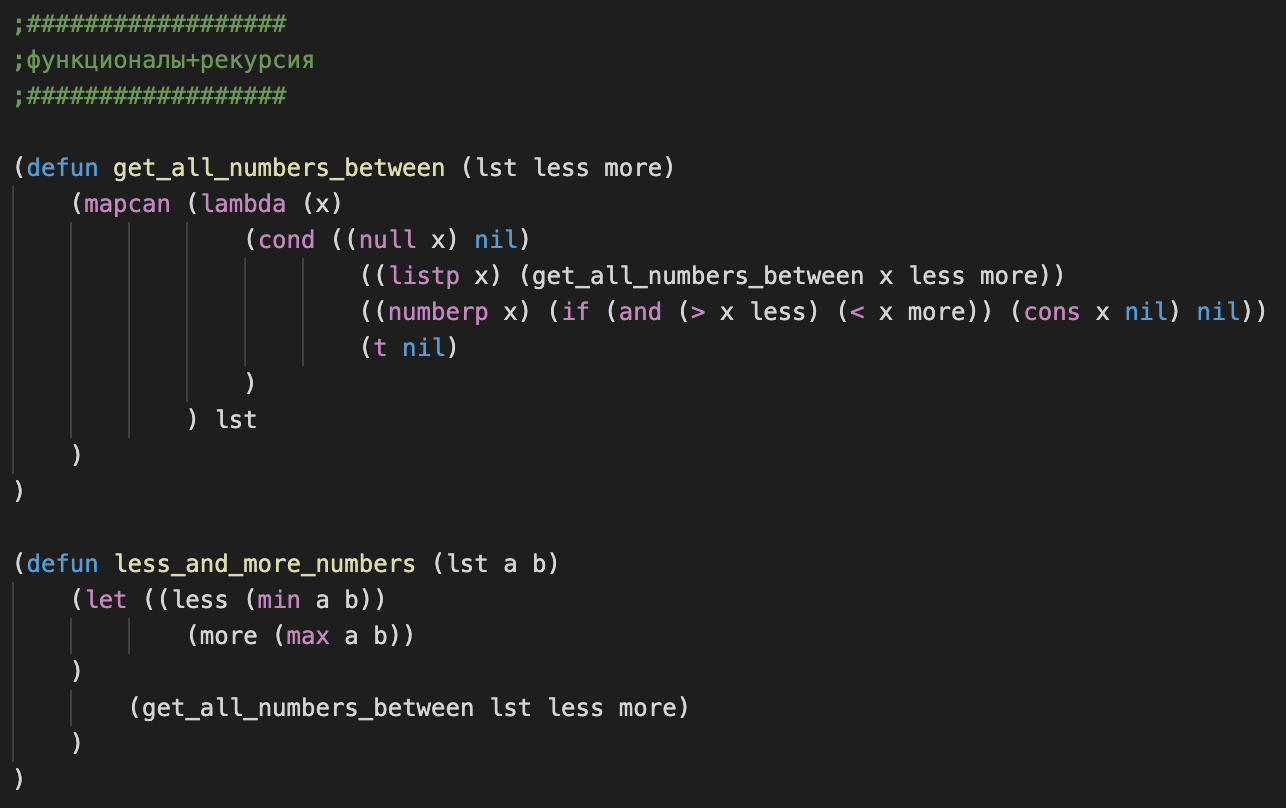
\includegraphics[scale = 0.8]{6.4.png}}
 			\label{ris:6.4}
 		\end{center}
 	\caption{Реализация функции, выбирающей из списка числа между двумя заданными границами, с использованием функционалов и рекурсии}
 	\end{figure}
 	
 	\subsection*{Назначение параметров функций}
 	
 	\begin{itemize}
 		\item Для реализации поставленной задачи используются функционалы и хвостовая рекурсия вместе, чтобы решить задачу наиболее оптимальным способом
 		\item Функция less\_and\_more\_numbers - главная функция, запускающая рекурсивную функцию less\_and\_more\_numbers с переданным ей списком lst и переменными less, more
 		\item Переменные less, more - минимальный и максимальные элементы из входных параметров a, b соответственно
 		\item В функции get\_all\_numbers\_between используется функционал mapcan, чтобы проходясь по всему списку lst, объединять полученный результат в результирующий список
 		\item Функции listp null и numberp - функции-проверки на nil, список и число соответственно
 	\end{itemize}
 	
 	\subsection*{Результаты работы}
 	
 	\begin{table} [h!]
 		\begin{center}
 			\begin{tabular}{|l|l|}
 				\hline
 				{\bf  Выражение} &    {\bf Результат} \\
 				\hline
 				{'(1 2 3 4 5 6 7 8 9) 3 7} & (4 5 6)\\
 				\hline
 				{'(1 2 3 4 5 6 7 8 9) 7 3} & (4 5 6)\\
 				\hline
 				{'(1 2 3 4 5 6 7 8 9) 3.3 4.3} & (4)\\
 				\hline
 				{'(1 2 3 4 5 6 7 8 9) 3.3 3.6} & NIL\\
 				\hline
 				{'(1 2 3 4 5 6 7 8 9) 10 13} & NIL\\
 				\hline
 				{'(1 2 3 4 5 6 7 8 9) -1 2.1} & (1 2)\\
 				\hline
 			\end{tabular}  
 			\label{m2}
 		\end{center}
 	\end{table}
 	
 	
 	\newpage
 	
 	\section*{6.5. Написать функцию, вычисляющую декартово произведение двух своих списков-аргументов. ( Напомним, что А х В это множество всевозможных пар (a b), где а принадлежит А, принадлежит В.)
 	}
 	
 	\subsection*{Реализация задания}
 	
 	\begin{figure}[h!]
 		\begin{center}
 			{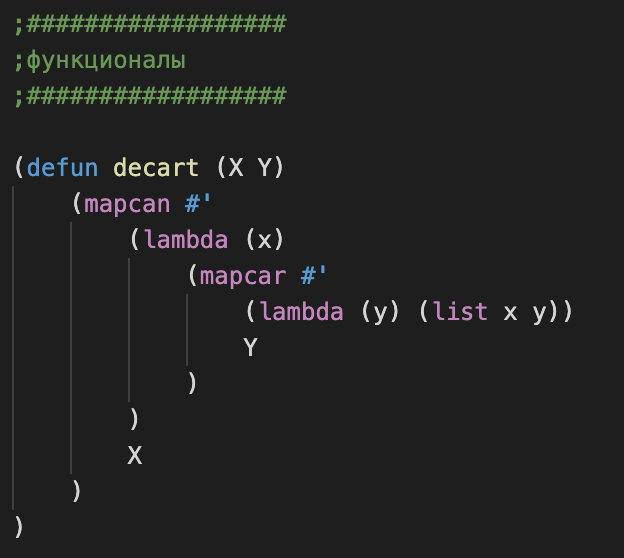
\includegraphics[scale = 0.9]{6.5f.png}}
 			\label{ris:6.5f}
 		\end{center}
 	\caption{Реализация функции, вычисляющей декартово произведение, с использованием функционалов}
 	\end{figure}
 
 
  	\begin{figure}[h!]
 	\begin{center}
 		{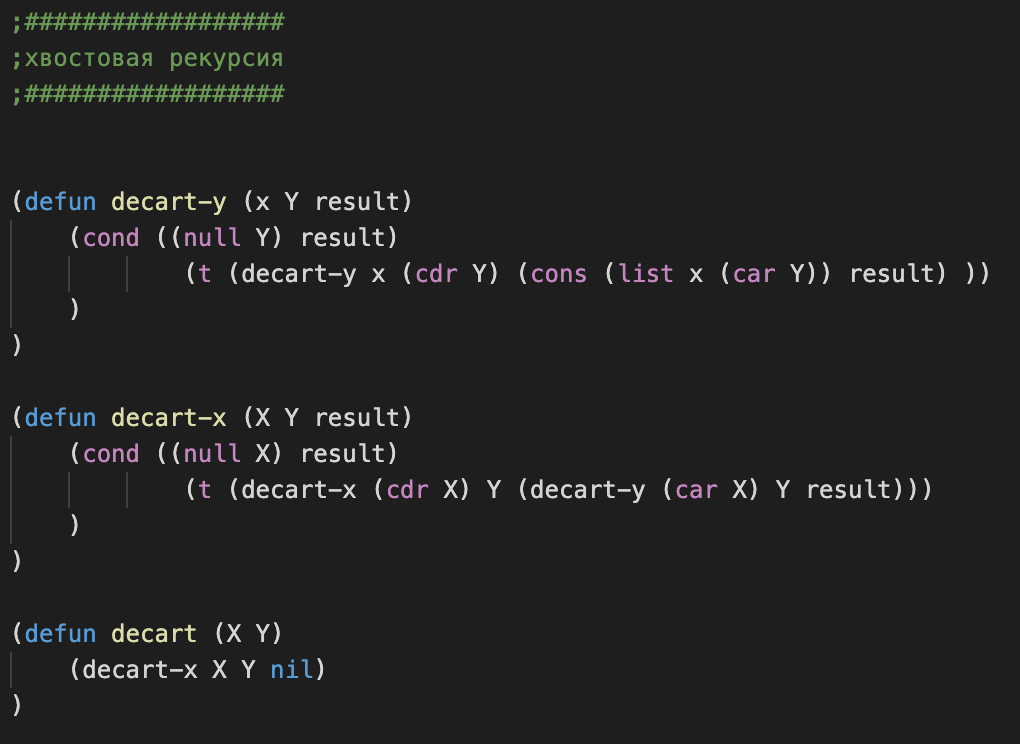
\includegraphics[scale = 0.7]{6.5r.png}}
 		\label{ris:6.5r}
 	\end{center}
 \caption{Рекурсивная реализация функции, вычисляющей декартово произведение, с использованием функционалов}
 \end{figure}

	\newpage
 	
 	\subsection*{Назначение параметров функций}
 	
 	\begin{itemize}
 		\item Функция decart, написанная с помощью функционалов проходится сначала по всем элементам списка X с помощью функционала mapcan и конкатенирует полученные списки в один список
 		\item Затем, "во внутреннем цикле", она проходится по всем элементам списка Y, объединяя полученные пары в списки из двух элементов
 		\item Рекурсивная реализация использует обертку - функцию decart, запускающую рекурсивную функцию decart-x с начальным результатом nil
 		\item В свою очередь функция decart-x запускает рекурсивную функцию decart-y для каждого элемента из списка X
 	\end{itemize}
 	
 	\subsection*{Результаты работы}
 	
 	 	Функции, реализованные с помощью функционалов и с помощью хвостовой рекурсии выдают одинаковые результаты на одних и тех же параметрах:
 	
 	\begin{table} [h!]
 		\begin{center}
 			\begin{tabular}{|l|l|}
 				\hline
 				{\bf  Выражение} & {\bf Результат} \\
 				\hline
 				{'(1 2 3) '(a b c)} & ((1 A) (1 B) (1 C) (2 A) (2 B) (2 C) (3 A) (3 B) (3 C))\\
 				\hline
 				{'(1 2 3) '(a b)} & ((1 A) (1 B) (2 A) (2 B) (3 A) (3 B))\\
 				\hline
 				{'(1 2) '(a b c)} & ((1 A) (1 B) (1 C) (2 A) (2 B) (2 C))\\
 				\hline
 				{'(1 2 3) '()} & NIL\\
 				\hline
 				{'() '(a b c)} & NIL\\
 				\hline
 			\end{tabular}  
 			\label{m2}
 		\end{center}
 	\end{table}
 	
 	
 	\section*{6.6. Почему так реализовано reduce, в чем причина?
 	}
 
 	\textit{(reduce \#'+ '()) -> 0}
 	\textit{(reduce \#'* '()) -> 1}
 	
 	Причина:
 	\textit{Если подпоследовательность пуста, а начальное значение не задано, то функция вызывается с нулевыми аргументами, а функция reduce возвращает то, что делает функция. Это единственный случай, когда функция вызывается не с двумя аргументами.}~\cite{reduce}
 	
 	Таким образом, функции + и *, вызывающиеся без аргументов, возвращают 0 и 1, сответственно.
 	
 	
 	\section*{Выводы}
 	
 	По итогу можно сделать вывод, что рекурсивные реализации функций будут работать чуть эффективней, чем функции, использующие функционалы, так как функционалы будут тратить время на вызов дополнительных функций.
 	
 	\section*{Ответы на вопросы}
 	
 	\subsection*{Способы организации повторных вычислений в Lisp:}
 	
 	\begin{enumerate}
 		\item Использование функционалов.
 		\item Использование рекурсиии.
 	\end{enumerate}
 	
 	\subsection*{Различные способы использования функционалов.}
 	
 	Функционалы:
 	
 	\begin{enumerate}
 		\item  Применяющие – однократное применение функции, являющейся аргументом, к остальным аргументам. Примеры применяющих функционалов: \textit{apply}, \textit{funcall}.
 		\item Отображающие – многократное применение функции, являющейся аргументом, к остальным аргументам по верхнему уровню. Примеры отображающих функционалов: \textit{mapcar}, \textit{reduce}, \textit{maplist}, \textit{mapcan}.
 	\end{enumerate}
 	
 	\subsection*{Что такое рекурсия?}
 	
 	\textit{Рекурсия} – это ссылка на определяемый объект во время его определения.
 	
 	\subsection*{Способы организации рекурсивных функций:}
 	
 	\begin{enumerate}
 		\item Хвостовая рекурсия.
 		\item Рекурсия по нескольким параметрам.
 		\item Дополняемая рекурсия.
 		\item Множественная рекурсия.
 	\end{enumerate}
 	
 	\subsection*{Способы повышения эффективности реализации рекурсии.}
 	
 	В целях повышения эффективности рекурсивных функций рекомендуется
 	формировать результат не на выходе из рекурсии, а на входе в рекурсию, все
 	действия выполняя до ухода на следующий шаг рекурсии. Это и есть хвостовая
 	\textit{рекурсия}.
 	
 	Для превращения не хвостовой рекурсии в хвостовую и в целях формирования результата (результирующего списка) на входе в рекурсию рекомендуется
 	использовать дополнительные (рабочие) параметры. При этом становится необходимым создать функцию-оболочку для реализации очевидного обращения к
 	функции.
 	
 	\addcontentsline{toc}{section}{Список литературы}
 	\begin{thebibliography}{}
 		
 	\bibitem{reduce} Common Lisp HyperSpec tm [Электронный ресурс]. – Режим доступа: http://clhs.lisp.se/Body/f\_reduce.htm, свободный. (Дата обращения: 28.03.2020 г.)
 	
 	\end{thebibliography}
 	
\end{document}